\subsection{実際のステッパ}
\label{実装-実際のステッパ}

実際に著者らが実装するステッパは、対象を OCaml の一部としており、以下の構文に対応している(一部は開発中である)。
\begin{itemize}
\item 整数、実数、真偽値、文字、文字列、リスト、組、レコード、ユーザ定義型
\item 条件分岐、変数定義、再帰関数定義、パターンマッチ、例外処理
\item List モジュール、ユーザ定義モジュール
\item 配列、逐次実行、標準出力関数(開発中)
\end{itemize}

副作用に関わる構文について、incremental でないステッパ\cite{FSA18}ではステッパプロセスが書き換え可能な変数の値や標準出力された文字列を保持することができたが、incremental にすることでそれが不可能になるので、プログラムの attribute を用いてそのような情報もステップ出力に含めるようにすることで実装することを目指している。

\begin{figure}
  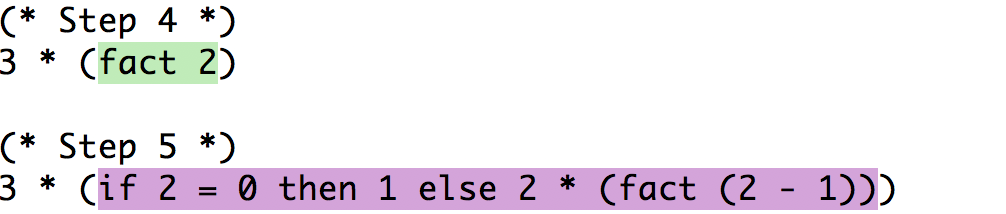
\includegraphics[height=2cm]{skip1.png}
  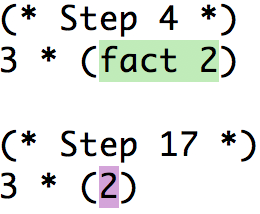
\includegraphics[height=2cm]{skip2.png}
  \caption{ステッパのスキップ機能}
  \label{figure:skip}
\end{figure}

また、著者らの incremental でないステッパ\cite{FSA18}は、プログラムの流れを理解する助けやステッパの利便性の向上のため、関数適用式が値に計算されるまでが1ステップであるかのように進める機能を有していた。図\ref{figure:skip} の左のように関数適用が簡約されるステップで Skip ボタンを押すと、図\ref{figure:skip} 右のように、下のプログラムが「関数適用式が値に簡約されたステップ」のプログラムに変わる。この状態で Next ボタンを押すとその続き、図\ref{figure:skip} の場合には \texttt{3 * 2 $\leadsto$ 6} のステップが表示される。これを本研究の incremental なステッパでも1ステップとして扱い、1度の実行で関数適用が値になるステップまでを計算し、その最後のステップを出力するように実装を進めている。そのためには、図\ref{figure:mode} の \texttt{mode} 型にスキップのためのコンストラクタを追加し、そのモードの場合には「実行している関数適用式が値になるステップまでは出力・終了を行わない」ようにするだけで良い。
